\documentclass{exam}

\usepackage{units} 
\usepackage{graphicx}
\usepackage[fleqn]{amsmath}
\usepackage{cancel}
\usepackage{float}
\usepackage{mdwlist}
\usepackage{booktabs}
\usepackage{cancel}
\usepackage{polynom}
\usepackage{caption}
\usepackage{fullpage}
\usepackage{comment}
\usepackage{enumerate}
\usepackage{xfrac}

\newcommand{\degree}{\ensuremath{^\circ}} 
\everymath{\displaystyle}

% \begin{figure}[H]
%   \centering
%   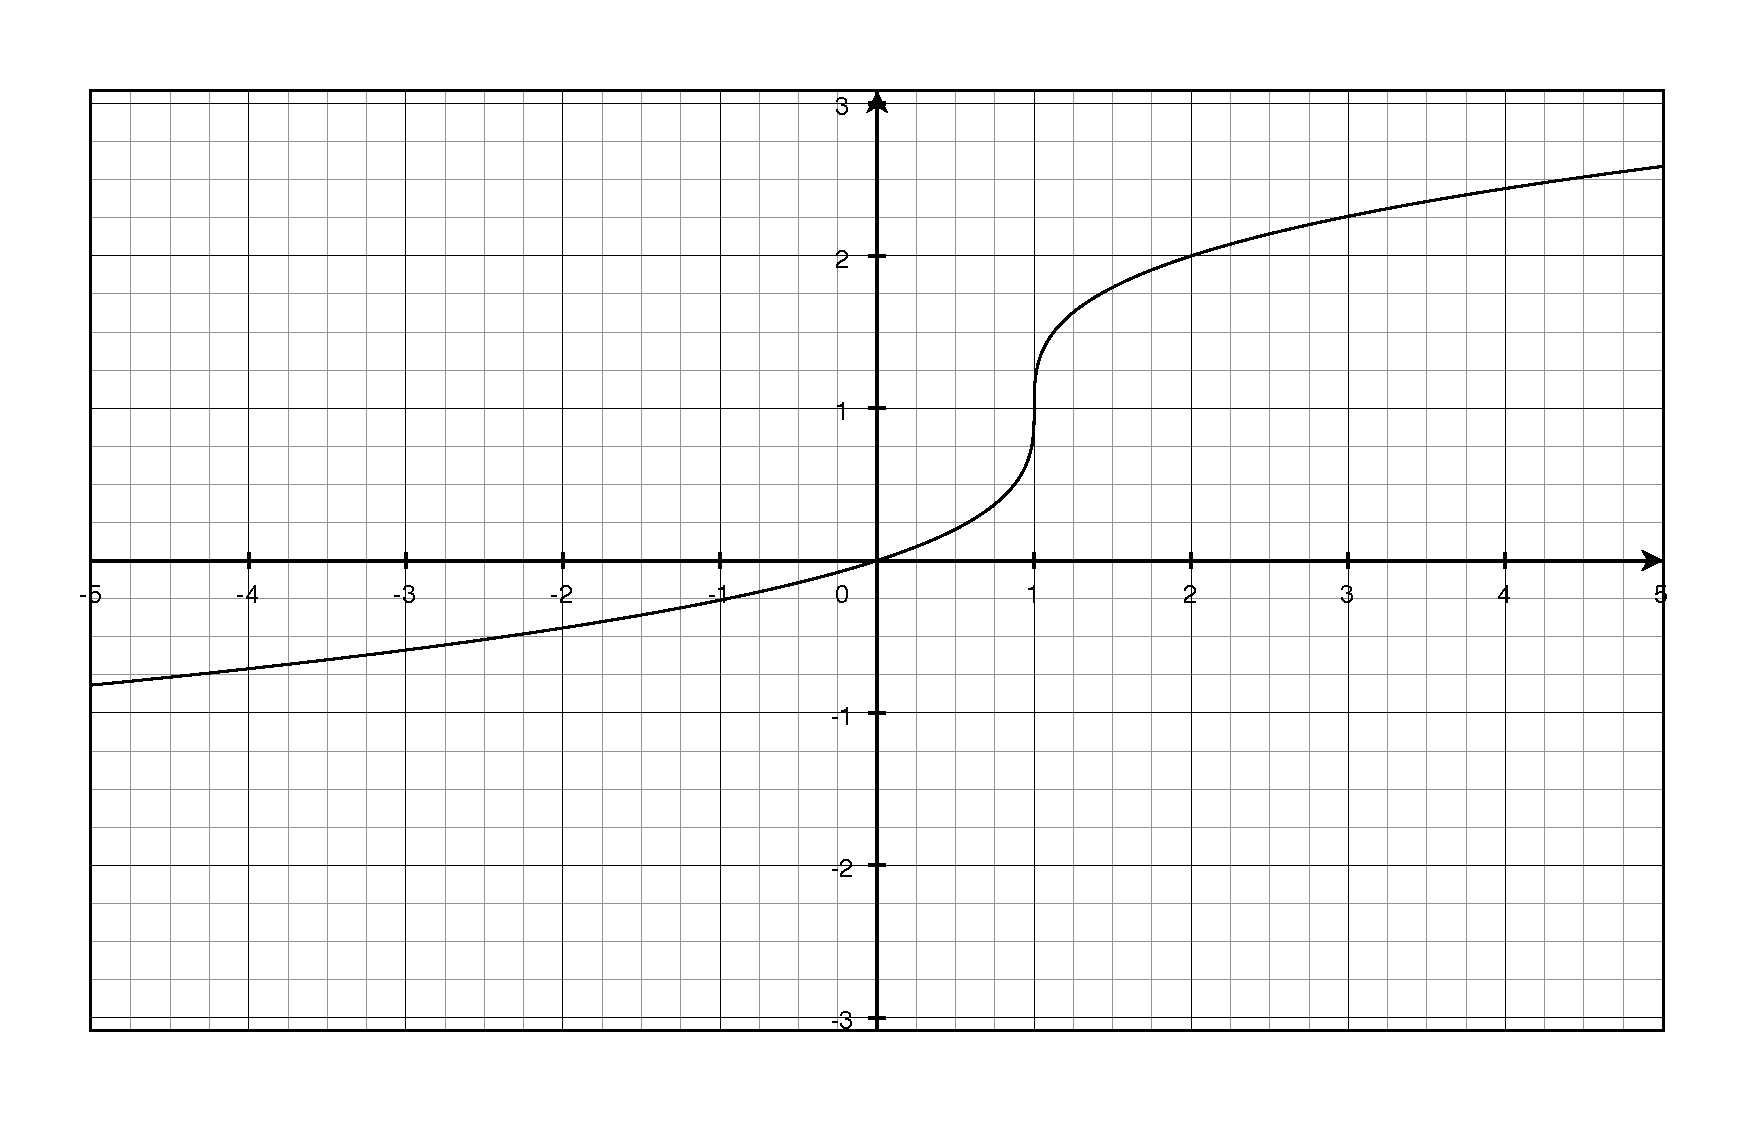
\includegraphics[scale=.3]{question7.eps}
%   \caption*{question 7}
% \end{figure}

% \begin{tabular}{cc}
%   \toprule
%   period & amplitude \\
%     $\pi$ & $2$ \\
%   \bottomrule
% \end{tabular}

\printanswers
\excludecomment{comment}

\ifprintanswers 
  \usepackage{2in1, lscape} 
\fi

\author{}
\date{\today}
\title{Math 142 \\ Homework Seven}

\begin{document}

  \maketitle

  \section{Homework}
  Section 6.2: 

  \section{Extra Credit}
  Section 6.2: TO DO

  \ifprintanswers

    \section{Section 6.1}
    \begin{description}

      \item[1] 
        \begin{tabular}[H]{cccccc}
          \toprule
          $\sin$         & $\cos$         & $\tan$         & $\sec$         & $\csc$         & $\cot$ \\
          % \midrule
          $\sfrac{4}{5}$ & $\sfrac{3}{5}$ & $\sfrac{4}{3}$ & $\sfrac{5}{3}$ & $\sfrac{5}{4}$ & $\sfrac{3}{4}$ \\
          \bottomrule
        \end{tabular}

      \item[2] 
        \begin{tabular}[H]{cccccc}
          \toprule
          $\sin$          & $\cos$           & $\tan$          & $\sec$           & $\csc$          & $\cot$ \\
          % \midrule
          $\sfrac{7}{25}$ & $\sfrac{24}{25}$ & $\sfrac{7}{24}$ & $\sfrac{25}{24}$ & $\sfrac{25}{7}$ & $\sfrac{24}{7}$ \\
          \bottomrule
        \end{tabular}

    \end{description}

  \else
    \vspace{1 cm}
    \begin{quote}
      \begin{em}
        TO DO
      \end{em}
    \end{quote}
    \hspace{1 cm} --Shunryu Suzuki
  \fi

\end{document}

